\documentclass[11pt]{article} % use larger type; default would be 10pt

\usepackage[utf8]{inputenc} % set input encoding (not needed with XeLaTeX)

%%% PAGE DIMENSIONS
\usepackage{geometry} % to change the page dimensions
\geometry{a4paper} % or letterpaper (US) or a5paper or....
% \geometry{margins=2in} % for example, change the margins to 2 inches all round
% \geometry{landscape} % set up the page for landscape
% read geometry.pdf for detailed page layout information

\usepackage{graphicx} % support the \includegraphics command and options

\usepackage[parfill]{parskip} % Activate to begin paragraphs with an empty line rather than an indent

%%% PACKAGES
\usepackage{amssymb}
\usepackage{booktabs} % for much better looking tables
\usepackage{array} % for better arrays (eg matrices) in maths
\usepackage{paralist} % very flexible & customisable lists (eg. enumerate/itemize, etc.)
\usepackage{verbatim} % adds environment for commenting out blocks of text & for better verbatim
\usepackage{subfig} % make it possible to include more than one captioned figure/table in a single float
% These packages are all incorporated in the memoir class to one degree or another...

%%% HEADERS & FOOTERS
\usepackage{fancyhdr} % This should be set AFTER setting up the page geometry
\pagestyle{fancy} % options: empty , plain , fancy
\renewcommand{\headrulewidth}{0pt} % customise the layout...
\lhead{}\chead{}\rhead{}
\lfoot{}\cfoot{\thepage}\rfoot{}

%%% END Article customizations

%%% The "real" document content comes below...

\title{Comp Methods Project I}
\author{Joe Sinotte}
%\date{} % Activate to display a given date or no date (if empty),
% otherwise the current date is printed

\begin{document}
\maketitle

\pagebreak
\tableofcontents
\pagebreak

\section{Problem Statement}

I have been given two sets of data, Ytrain and Ytest. Each data set contains 200 images of 40 individuals, with 5 images of each individual.

Problem: With the given data, is it possible to code a matlab program to match images from Ytrain to an individual in Ytest? 
\section{Methodology}

\subsection{Dimension Reduction}
Since image data are usually very large, it can be beneficial to reduce the dimensionality of the data to make the program less computationally expensive. There are various methods to reduce dimensionality. This paper shall use two of these methods, which will be described in greater below.

The first approach to dimension reduction that will be discussed is Principal Component Analysis (PCA). The steps of PCA are as follows:
\begin{enumerate}
\item Find the sample covariance matrix, $C\in\mathbb{R}^{n \times n}$, of the data.
\item Compute the singular value decomposition of C, which yields the orthogonal matrix $UPCA\in\mathbb{R}^{n \times n}$.
\item Select the first k columns of U and denote them by the matrix $UPCA$.
\item Define a transformation of the data as $Z=(UPCA)'^{*}Ytrain$. Where, $Z \in\mathbb{R}^{m \times k}$
\end{enumerate}

In addition, a feature vector is formed by applying the same transformation to a randomly chosen column vector from Ytest, denoted as I. Hence,
\begin{center}
$Z1=(UPCA)'^{*}I$
\end{center}

This method provides the benefit of only retaining the k dimensions with the most explanatory power, and all of the superfluous dimensions are omitted from the rest of the process, decreasing the computational expense of the entire procedure.

The second method that will be examined is the Simple Projection (SP) method. In this method, a transformation is derived by selecting the first k columns of an identity matrix which, in this example, is of dimension $(s_{1} \times s_{2})=644$, and defining the newly acquired matrix as $USP$. Thus, the transformation can be expressed as:
\begin{center}
$Y1=(USP)'^{*}Ytrain$
\end{center}

With the feature vector,
\begin{center}
$I1=(UPCA)'^{*}I$
\end{center}

The SP method carries benefits and costs of its use. This method is simple and fast, making it a computationally cheap way to reduce data dimensionality. On the other hand, this method, in contrast to the PCA method, does not allow the user to only include the most descriptive dimensions. This means that in the process of reducing dimensionality, the transformation may omit the most informative portions of the data.
\subsection{Image Recognition}
Having successfully reduced the dimensionality of the images under scrutiny, I will now turn my attention to the method used to match a randomly selected column from I1 and Z1 to columns of Y1 and  Z, respectively. Here, I use the Nearest Neighbor Classifier to find the column of the Y1 that minimizes the normed distance between Y1 and I1, and likewise the column of Z that minimizes the normed distance between Z and Z1. The column that minimizes this distance in each case is called the nearest neighbor, and if that column corresponds to an image of the same individual 

The process described above was repeated for k equals one to forty dimensions. For each k, one hundred loops are run, and the proportion on correct identifications is calculated and defined as F(K).  

\section{Results}

Here, I will give a brief overview of the results of this exercise. Overall, the program was a success. Below, I have included examples of successful matches, both with SP and PCA.

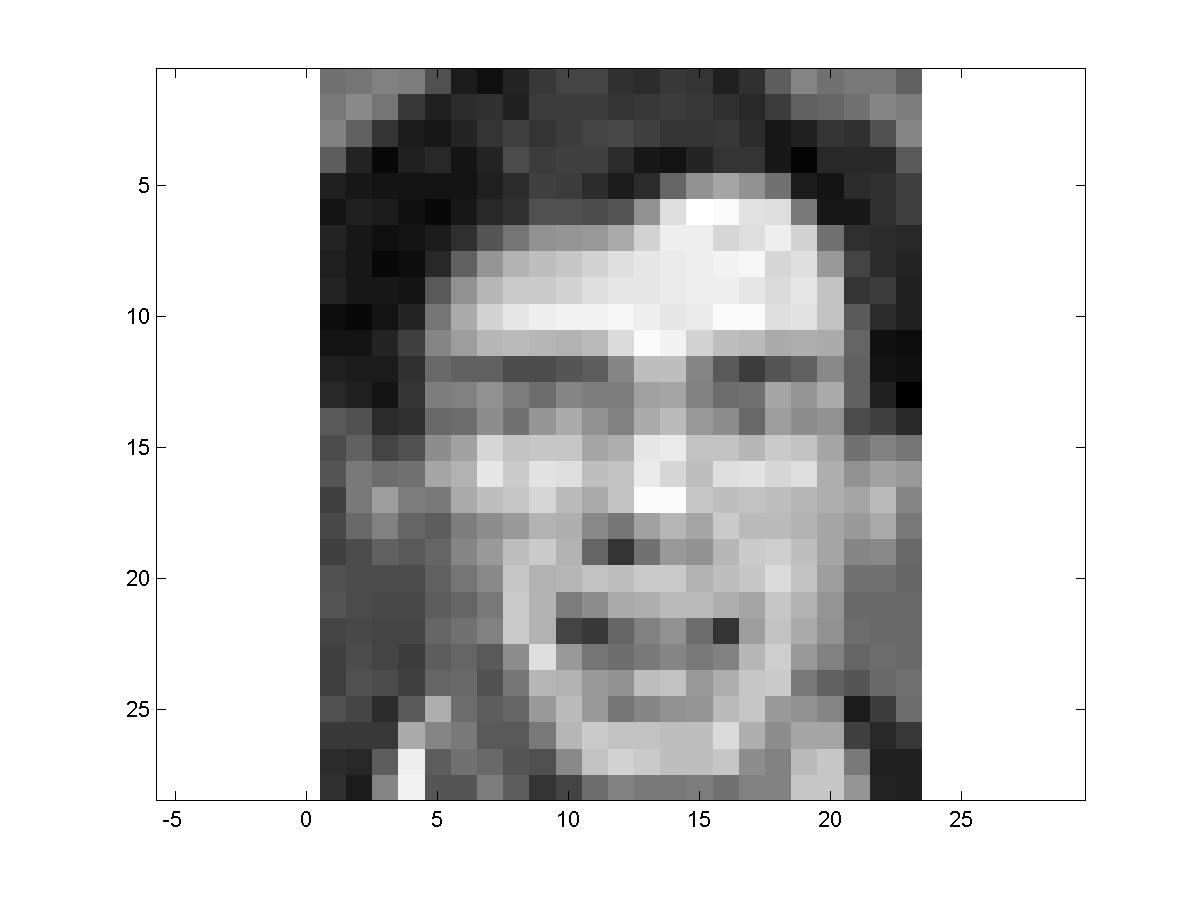
\includegraphics[scale=.17]{figure2}
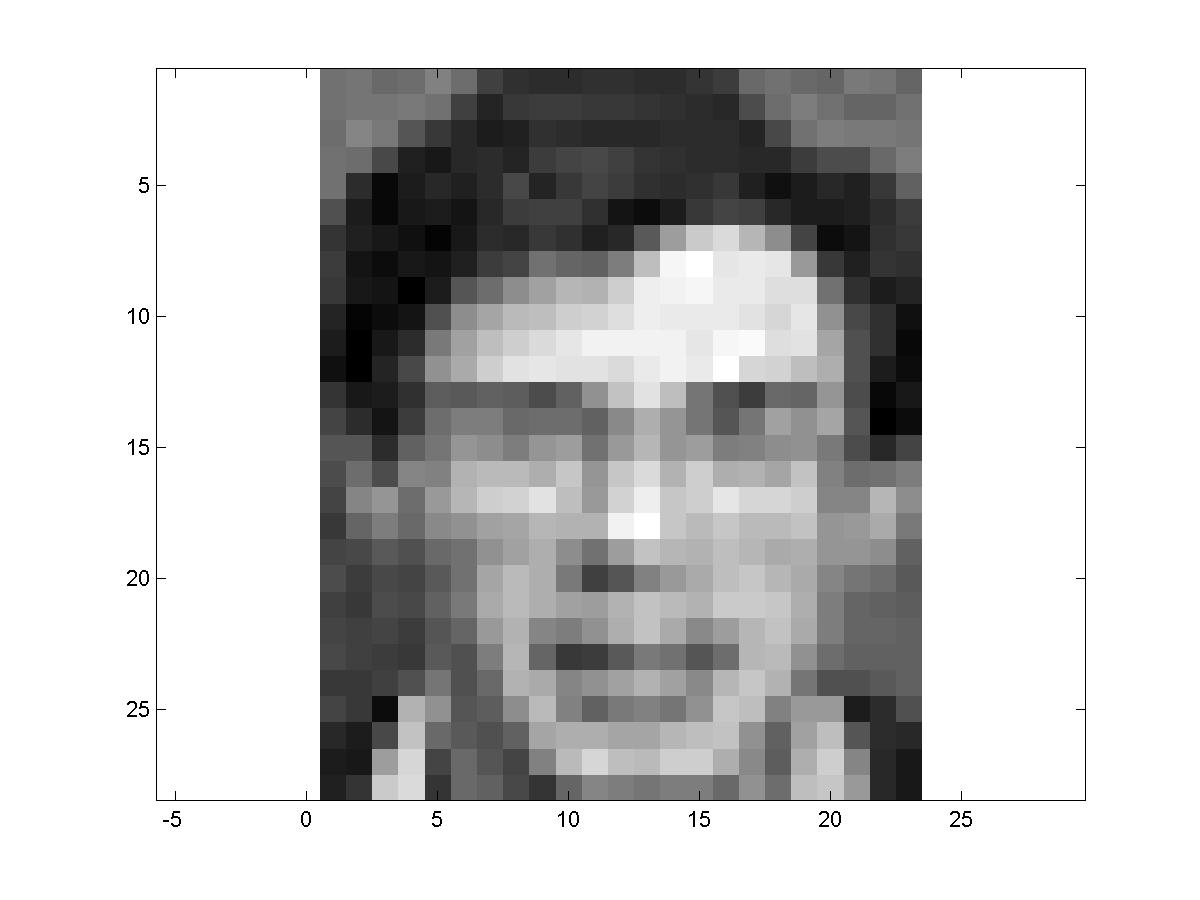
\includegraphics[scale=.17]{figure3}

This is an example of a match with a simple projection.

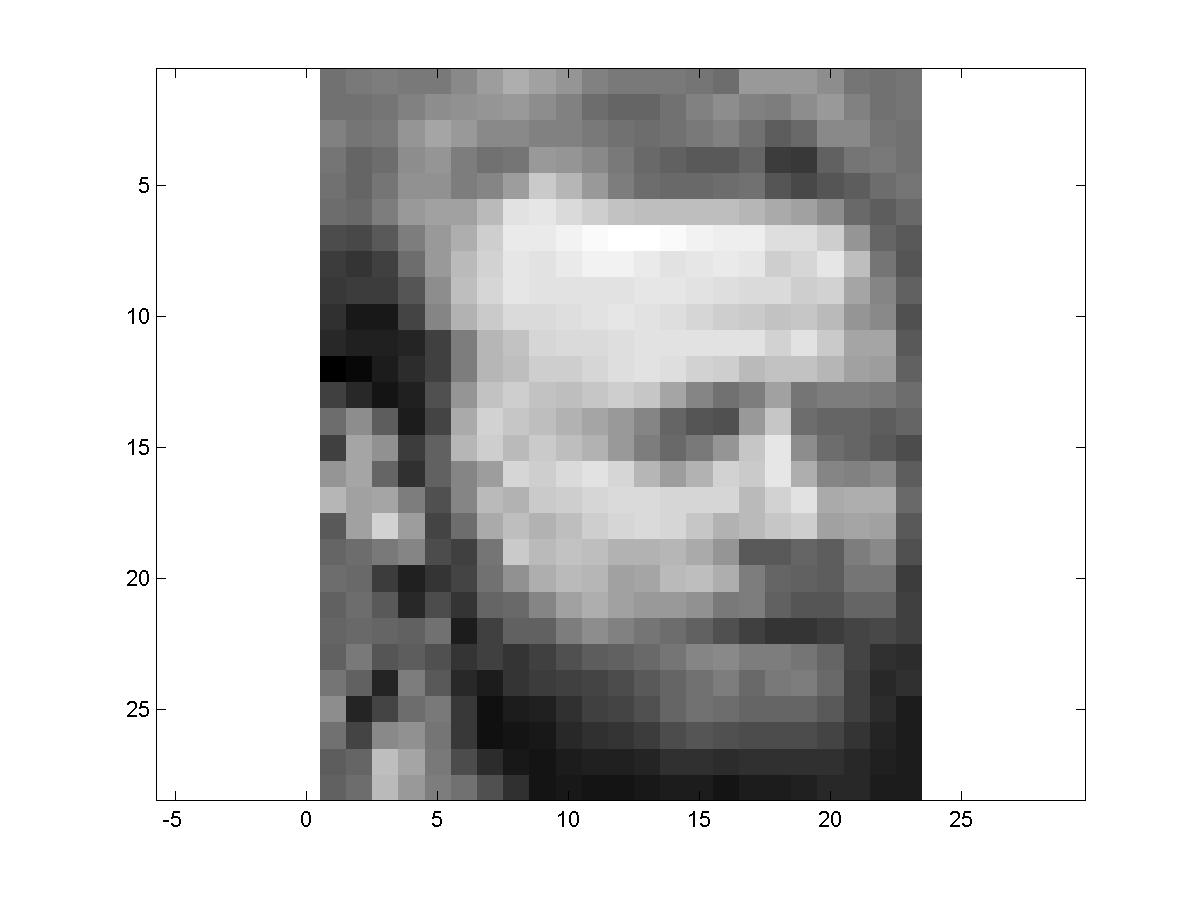
\includegraphics[scale=.17]{figure4}
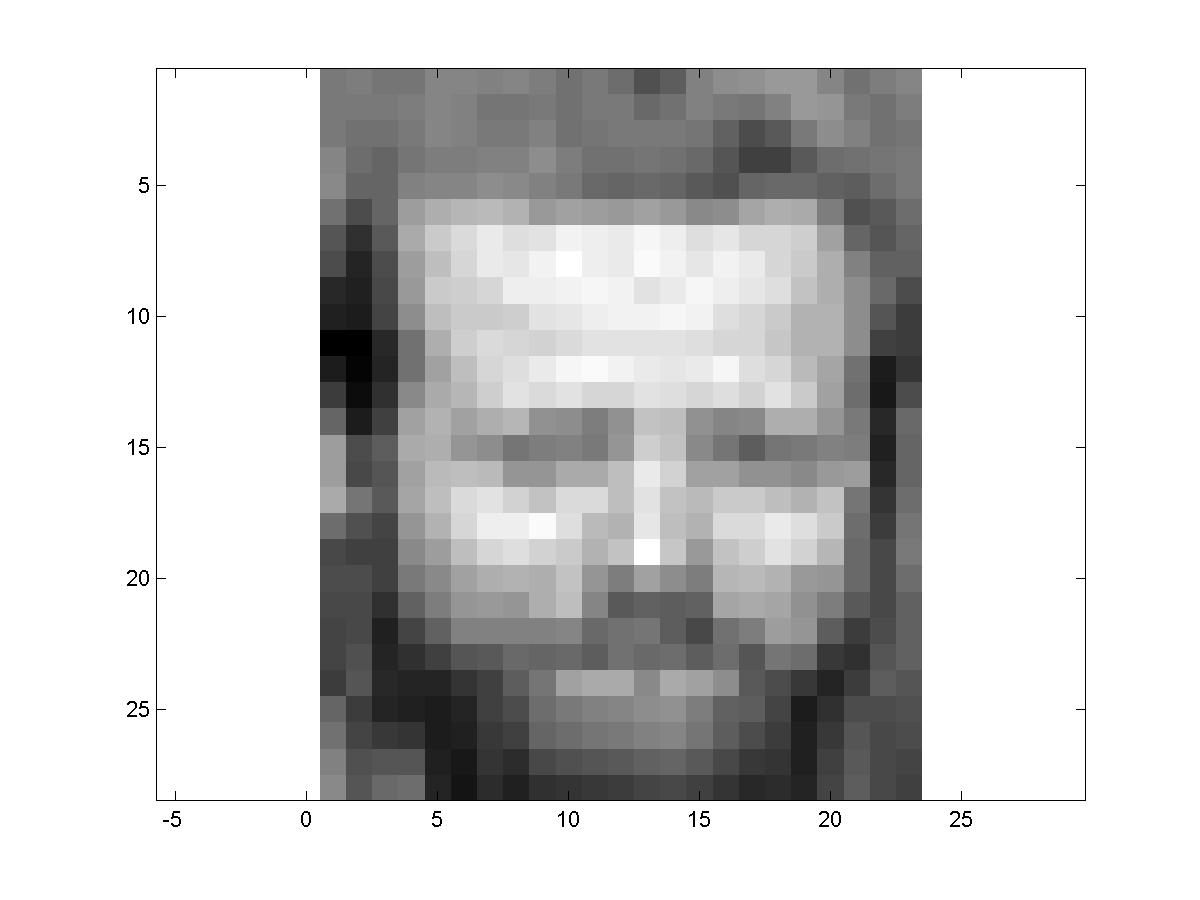
\includegraphics[scale=.17]{figure5}

This is an example of a match with PCA.

\vspace{4mm}

\begin{center}
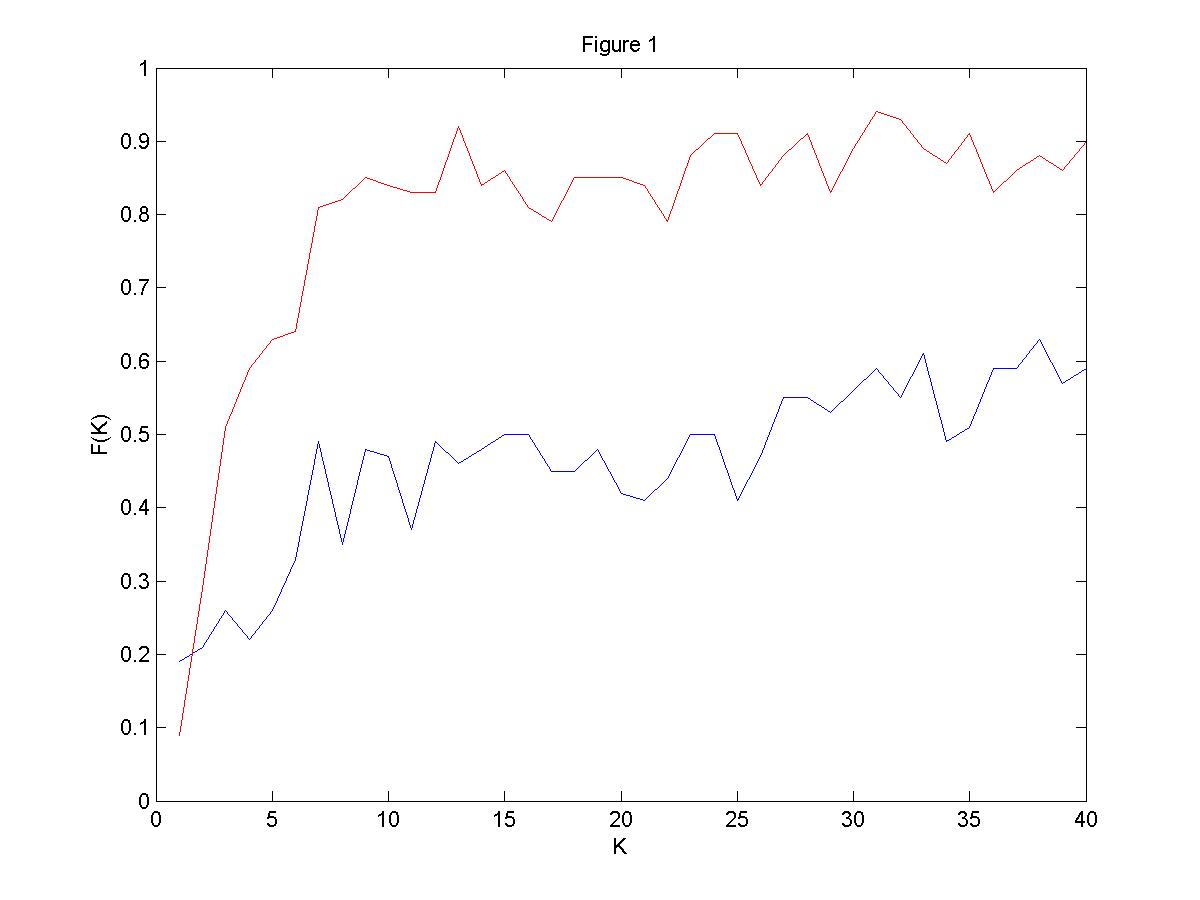
\includegraphics[scale=.3]{figure1}
\end{center}

Figure  1 displays the results of the exercise under discussion. The horizontal axis denotes the number of dimensions to which the data sets are being reduced, while the vertical axis displays the proportion of correct identifications for each value of k. As the figure shows, the simple projection method is more accurate for very small dimensional problems. As the number of dimensions increases, PCA becomes significantly more efficient, and consistently yield high match proportions. Thus, it can be concluded that PCA gives the most accurate results for higher dimensional problems.

It is also worth noting that the variation in F(K) is quite high with smaller K values. However, as we allow K to increase, F(K) becomes much more stable for both the simple projection and principal component methods.

In conclusion, I find the exercise a success, with a high proportion of matches under PCA and a lower proportion under SP.  

\section{Matlab Programs}

All programs are attached on a separate sheet.

\end{document}